\subsubsection{Feature extraction}
    Для извлечения из аудиодорожек признаков в виде эмбеддингов использовалась VGGish модель. Она заключается в следующем:
    \begin{enumerate}
        \item Конвертируем входной аудиофайл в мел-спектрограмму
        \item Применяем нейронную сеть VGGish
        \item Применяем PCA (метод главных компонент)
    \end{enumerate}
    
\subsubsection{Segmentation model}
    Расммотрим слои нашей модели:
    \begin{figure}[H]
        \centering
        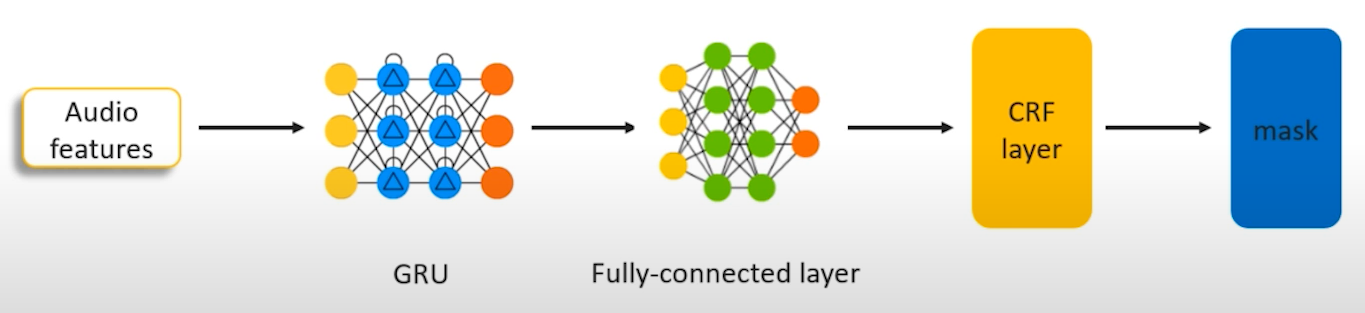
\includegraphics[scale=0.5]{images/model.PNG}
        \caption{Модель}
        \label{model}
    \end{figure}
    \begin{itemize}
        \item GRU (Gated Recurrent Units) - механизм управления рекуррентной сети
        \item Fully-connected layer - полносвязный слой
        \item CRF (Conditional Random Fields) - дискриминативная ненаправленная вероятностная графическая модель, являющаяся разновидностью марковских случайных полей (Markov Random Field), используемая для прогнозирования последовательностей
    \end{itemize}
